\documentclass{standalone}
\usepackage{tikz}
\usepackage{amsmath}
\usepackage{xcolor}
\usetikzlibrary{arrows.meta, decorations.pathreplacing, backgrounds, positioning, calc}

% Define custom colors
\definecolor{softyellow}{HTML}{F2D648}
\definecolor{dustyblue}{HTML}{9EB9D4}
\definecolor{berkeleyblue}{RGB}{0, 50, 98}
\definecolor{berkeleygold}{RGB}{253, 181, 21}
\definecolor{berkeleyblue}{RGB}{0, 50, 98}
\definecolor{berkeleygold}{RGB}{253, 181, 21}
\definecolor{berkeleylight}{RGB}{198, 217, 241} % Lighter blue for backgrounds
\begin{document}

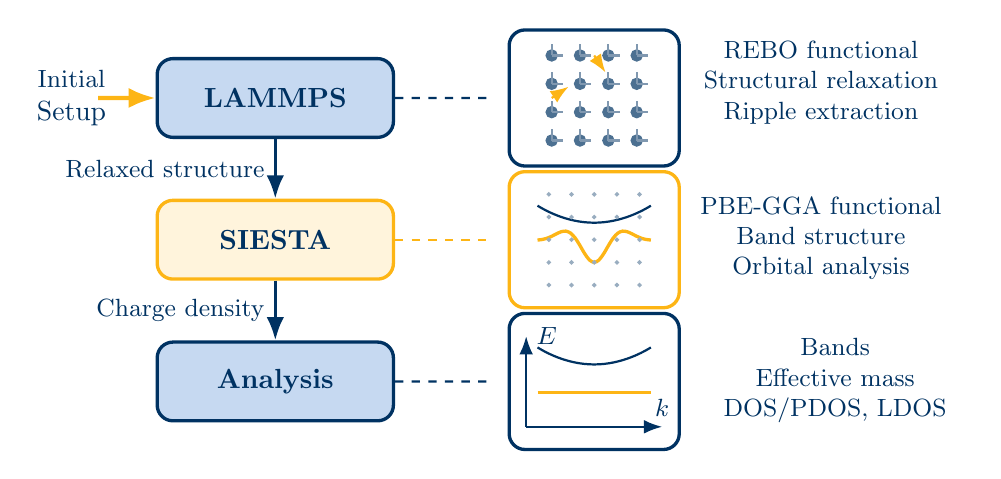
\begin{tikzpicture}[
  scale=0.9,
  >=Latex,
  box/.style={draw, rounded corners=2mm, very thick, minimum width=3cm, minimum height=1cm},
  bluebox/.style={box, fill=berkeleylight, text=berkeleyblue, draw=berkeleyblue, line width=1.2pt},
  goldbox/.style={box, fill=berkeleygold!15, text=berkeleyblue, draw=berkeleygold, line width=1.2pt},
  panel/.style={draw, rounded corners=2mm, very thick, line width=1.2pt},
  arrow/.style={->, line width=1.2pt}
]
  % Step 1: LAMMPS
  \node[bluebox] (lammps) at (0,2) {\textbf{LAMMPS}};
  
  % LAMMPS visualization
  \begin{scope}[shift={(4.5,2)}, scale=0.8]
    \draw[panel, berkeleyblue] (-1.5,-1.2) rectangle (1.5,1.2);
    \foreach \x in {-0.75,-0.25,0.25,0.75} {
      \foreach \y in {-0.75,-0.25,0.25,0.75} {
        \filldraw[berkeleyblue!70] (\x,\y) circle (0.1);
        \draw[berkeleyblue!50, thick] (\x,\y) -- (\x+0.2,\y);
        \draw[berkeleyblue!50, thick] (\x,\y) -- (\x,\y+0.2);
      }}
    \draw[berkeleygold, thick, -Latex] (-0.75,0) -- (-0.45,0.2);
    \draw[berkeleygold, thick, -Latex] (0,0.75) -- (0.2,0.45);
    
    \node[below=0cm, text=berkeleyblue] at (4, 1.25) {\small \begin{tabular}{c}REBO functional\\ Structural relaxation\\ Ripple extraction\end{tabular}};
  \end{scope}
  
  % Step 2: SIESTA  
  \node[goldbox] (siesta) at (0,0) {\textbf{SIESTA}};
  
  % SIESTA visualization
  \begin{scope}[shift={(4.5,0)}, scale=0.8]
    \draw[panel, berkeleygold] (-1.5,-1.2) rectangle (1.5,1.2);
    \draw[berkeleyblue, thick] (-1,0.6) parabola bend (0,0.3) (1,0.6);
      
    \draw[berkeleygold, very thick] plot[smooth, domain=-1:1]     
      (\x, {-0.4*exp(-3*\x*\x)*cos(5*\x*180/pi)});
      
    \foreach \x in {-0.8,-0.4,0,0.4,0.8} {
      \foreach \y in {-0.8,-0.4,0,0.4,0.8} {
        \filldraw[berkeleyblue!40] (\x,\y) circle (0.03);
      }}
      
    \node[below=0cm, text=berkeleyblue] at (4,1) {\small \begin{tabular}{c}PBE-GGA functional\\ Band structure\\ Orbital analysis\end{tabular}};
  \end{scope}
  
  % Step 3: Analysis
  \node[bluebox] (analysis) at (0,-2) {\textbf{Analysis}};
  
  % Analysis visualization
  \begin{scope}[shift={(4.5,-2)}, scale=0.8]
    \draw[panel, berkeleyblue] (-1.5,-1.2) rectangle (1.5,1.2);
    \draw[-Latex, berkeleyblue, thick] (-1.2,-0.8) -- (1.2,-0.8) node[above, text=berkeleyblue] {\small $k$};
    \draw[-Latex, berkeleyblue, thick] (-1.2,-0.8) -- (-1.2,0.8) node[right, text=berkeleyblue] {\small $E$};
    
    % Bands and flattening illustration
    \draw[berkeleyblue, thick] (-1,0.6) parabola bend (0,0.3) (1,0.6);
    \draw[berkeleygold, very thick] (-1,-0.2) -- (1,-0.2);
    
    \node[below=0cm, text=berkeleyblue] at (4.25,1) {\small \begin{tabular}{c}Bands\\ Effective mass\\ DOS/PDOS, LDOS\end{tabular}};
  \end{scope}
  
  % Connecting arrows between steps
  \draw[arrow, berkeleyblue] (lammps) -- (siesta) node[midway, left, text=berkeleyblue] {\small Relaxed structure};
  \draw[arrow, berkeleyblue] (siesta) -- (analysis) node[midway, left, text=berkeleyblue] {\small Charge density};
  
  % Feedback loop 
  \draw[arrow, berkeleygold, line width=1.5pt] (-2.5,2) -- (-2,2) -- (lammps.west);
  \node[anchor=east, align=center, text=berkeleyblue] at (-2.25,2) {\small Initial\\Setup};
  
  % Connecting lines between boxes and visualizations
  \draw[thick, dashed, berkeleyblue] (lammps.east) -- (3,2);
  \draw[thick, dashed, berkeleygold] (siesta.east) -- (3,0);
  \draw[thick, dashed, berkeleyblue] (analysis.east) -- (3,-2);
\end{tikzpicture}


\end{document}
